\vspace{-3mm}
Our experiments are divided into two parts. First, we evaluate our agent in a variety of existing long-term memory, generalization, and meta-learning environments. We then explore the combination of AMAGO's adaptive memory and hindsight instruction relabeling in multi-task domains with procedurally generated environments. Additional results, details, and discussion for each of our experiments can be found in Appendix \ref{app:experiment_details}. Unless otherwise noted, AMAGO uses a context length $l$ equal to the entire rollout horizon $H$. These memory lengths are not always necessary on current benchmarks, but we are interested in evaluating the performance of RL on long sequences so that AMAGO can serve as a strong baseline in developing new benchmarks that require more adaptation.

\subsection{Long-Term Memory, Generalization, and Meta-Learning}
\label{sec:experiments:metarl}

\begin{figure}[h!]
    \centering
    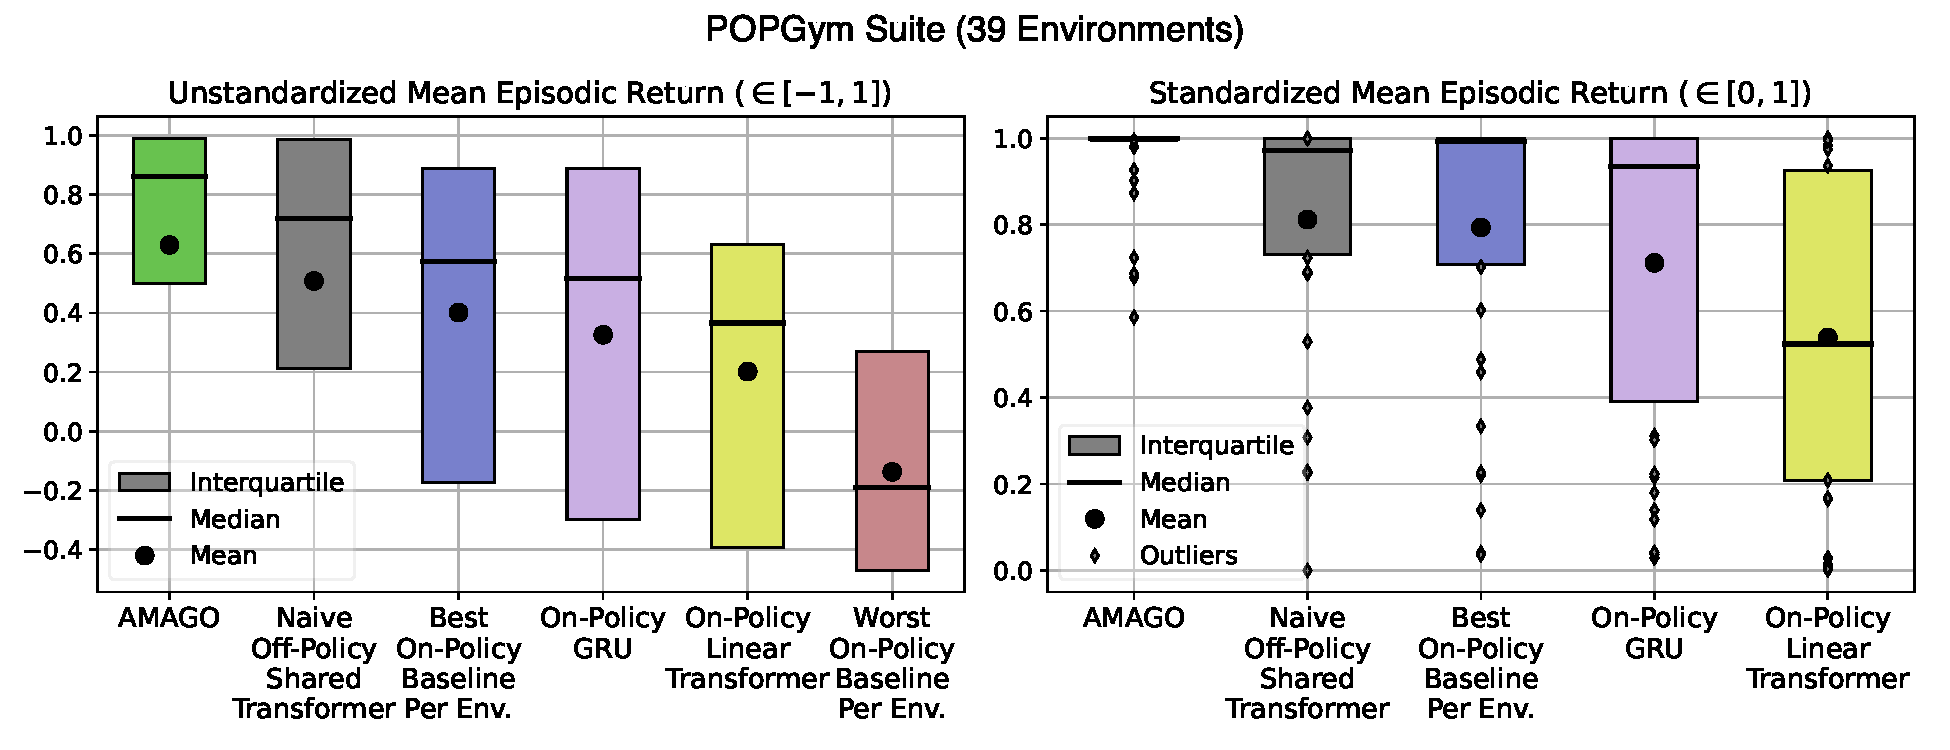
\includegraphics[width=.99\textwidth]{figs/popgym_summary_expanded_outliers.pdf}
    \caption{\textbf{Summary of POPGym Suite Results.} \textbf{(Left)} Aggregate results based on raw returns. \textbf{(Right)} Relative performance standardized by the highest and lowest scores in each environment.}
    \label{fig:popgym_summary}
\end{figure}



POPGym \cite{morad2023popgym} is a recent benchmark for evaluating long-term memory and generalization in a range of CMDPs. Performance in POPGym is far from saturated, and the challenges of sequence-based learning often prevent prior on-policy results from meaningfully outperforming memory-free policies. We tune AMAGO on one environment to meet the sample limit and architecture constraints of the original benchmark before copying these settings across $38$ additional environments. Figure \ref{fig:popgym_summary} summarizes results across the suite. We compare against the best existing baseline (a recurrent GRU-based agent \cite{cho2014learning}) and the most comparable architecture (an efficient Transformer variant \cite{katharopoulos_transformers_2020}). We also report the aggregated results of the best baseline in each environment --- equivalent to an exhaustive grid search over $13$ alternative sequence models trained by on-policy RL. If we standardize the return in each environment to $[0, 1]$ based on the highest and lowest baseline, as done in \cite{morad2023popgym}, AMAGO achieves an average score of $.95$ across the suite, making it a remarkably strong default for sequence-based RL. We perform an ablation that naively applies the shared Transformer learning update without AMAGO's other details --- such as our Transformer architecture and multi-gamma update. The naive baseline performs significantly worse, and the metrics in Figure \ref{fig:popgym_summary} mask its collapse in $9/39$ environments; AMAGO maintains stability in all of its $120+$ trials despite using model sizes and update-to-data ratios that are not tuned. Learning curves and additional experiments are listed in Appendix \ref{app:experiment_details:popgym}. 

\begin{figure}[h!]
    \centering
    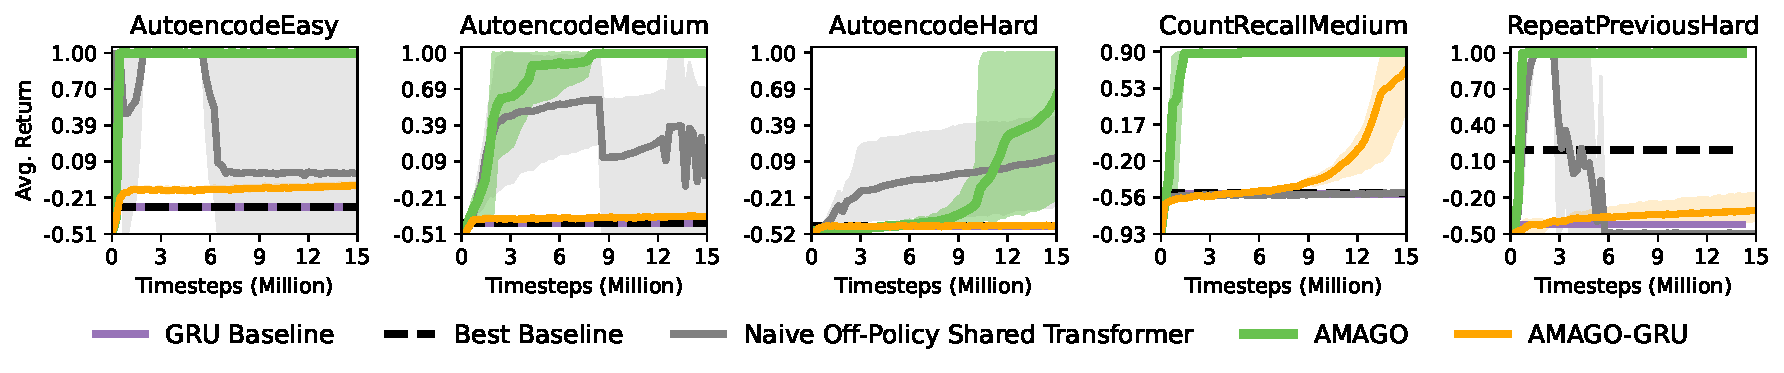
\includegraphics[width=\textwidth]{figs/popgym_vs_rnn_condensed.pdf}
    \vspace{-8mm}
    \caption{\textbf{Memory-Intensive POPGym Environments.} AMAGO's off-policy updates can improve performance in general, but its Transformer turns hard memory-intensive environments into a straightforward recall exercise. Appendix \ref{app:experiment_details:popgym} reports results on more than $30$ additional environments.\vspace{-4mm}}
    \label{fig:popgym_memory_curves}
\end{figure}

Much of AMAGO's performance gain in POPGym appears to be due to its ability to unlock Transformers' memory capabilities in off-policy RL: there are $9$ recall-intensive environments where the GRU baseline achieves a normalized score of $.19$ compared to AMAGO's $.999$. Figure \ref{fig:popgym_memory_curves} ablates the impact of AMAGO's trajectory encoder from the rest of its off-policy details by replacing its Transformer with a GRU-based RNN in a sample of these recall-intensive environments.

We test the limits of AMAGO's recall using a ``Passive T-Maze'' environment from concurrent work \cite{ni2023transformers}, which creates a way to isolate memory capabilities at any sequence length. Solving this task requires accurate recall of the first timestep at the last timestep $H$. AMAGO trains a single RL Transformer to recover the optimal policy until we run out of GPU memory at context length $l = H = 10,000$ (Figure \ref{fig:case_studies} top right). One concern is that AMAGO's maximum context lengths, large policies, and long horizons may hinder performance on easier problems where they are unnecessary, leading to the kind of hyperparameter tuning we would like to avoid. We demonstrate AMAGO on two continuous-action meta-RL problems from related work with dense (Fig. \ref{fig:case_studies} left) and sparse (Fig. \ref{fig:case_studies} bottom right) rewards where performance is already saturated, with strong and stable results. 

\begin{figure}[h!]
    \centering
    \vspace{-2mm}
    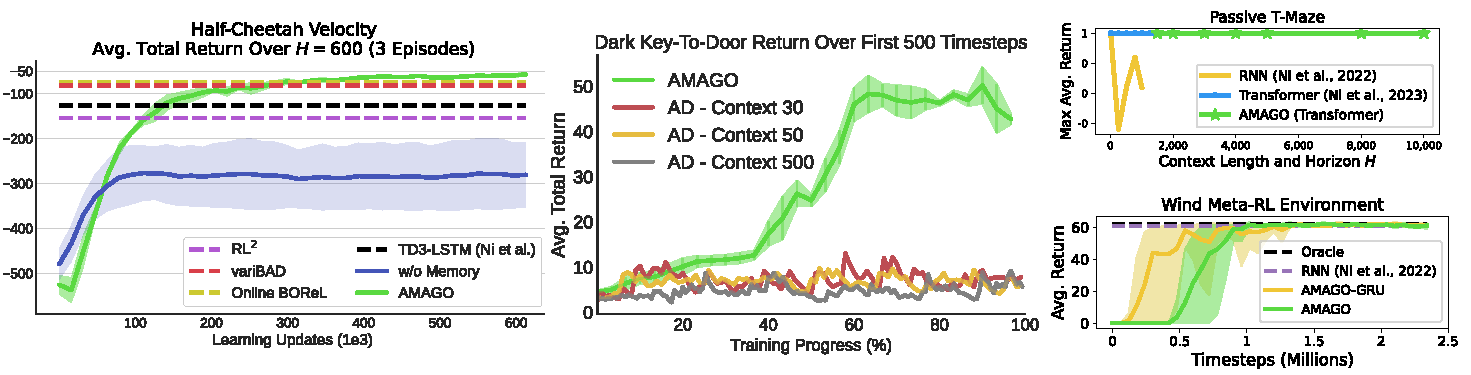
\includegraphics[width=\textwidth]{figs/case_studies_arxivV2_iclrV2.pdf}
    \vspace{-6mm}
    \caption{\textbf{Case Studies in In-Context Adaptation.} \textbf{(Left)} Adaptation over three episodes in Half-Cheetah Velocity \cite{finn2017model}. \textbf{(Center)} AMAGO vs. Algorithm Distillation over the first 500 timesteps of Dark Key-To-Door \cite{laskin2022context}. \textbf{(Bottom Right)} Adaptation to a sparse-reward environment with continuous actions \cite{ni2022recurrent}. \textbf{(Top Right)} AMAGO solves the Passive T-Maze memory experiment \cite{ni2023transformers} up until the GPU memory limit of $l = H = 10,000$ timesteps.\vspace{-2mm}}
    \label{fig:case_studies}
\end{figure}

Like several recent approaches that reformulate RL as supervised learning (Sec. \ref{sec:related}), AMAGO scales with the size and sequence length of a single Transformer. However, it creates a stable way to optimize its Transformer on the true RL objective rather than a sequence modeling loss. This can be an important advantage when the supervised objective becomes misaligned with our true goal. For example, we replicate Algorithm Distillation (AD) \cite{laskin2022context} on a version of its Dark Key-To-Door meta-learning task. AMAGO's ability to successfully optimize the return over any horizon $H$ lets us control sample efficiency at test-time (Fig. \ref{fig:case_studies} center), while AD's adaptation rate is limited by its dataset and converges several thousand timesteps later in this case. 


\begin{figure}[h!]
    \centering
    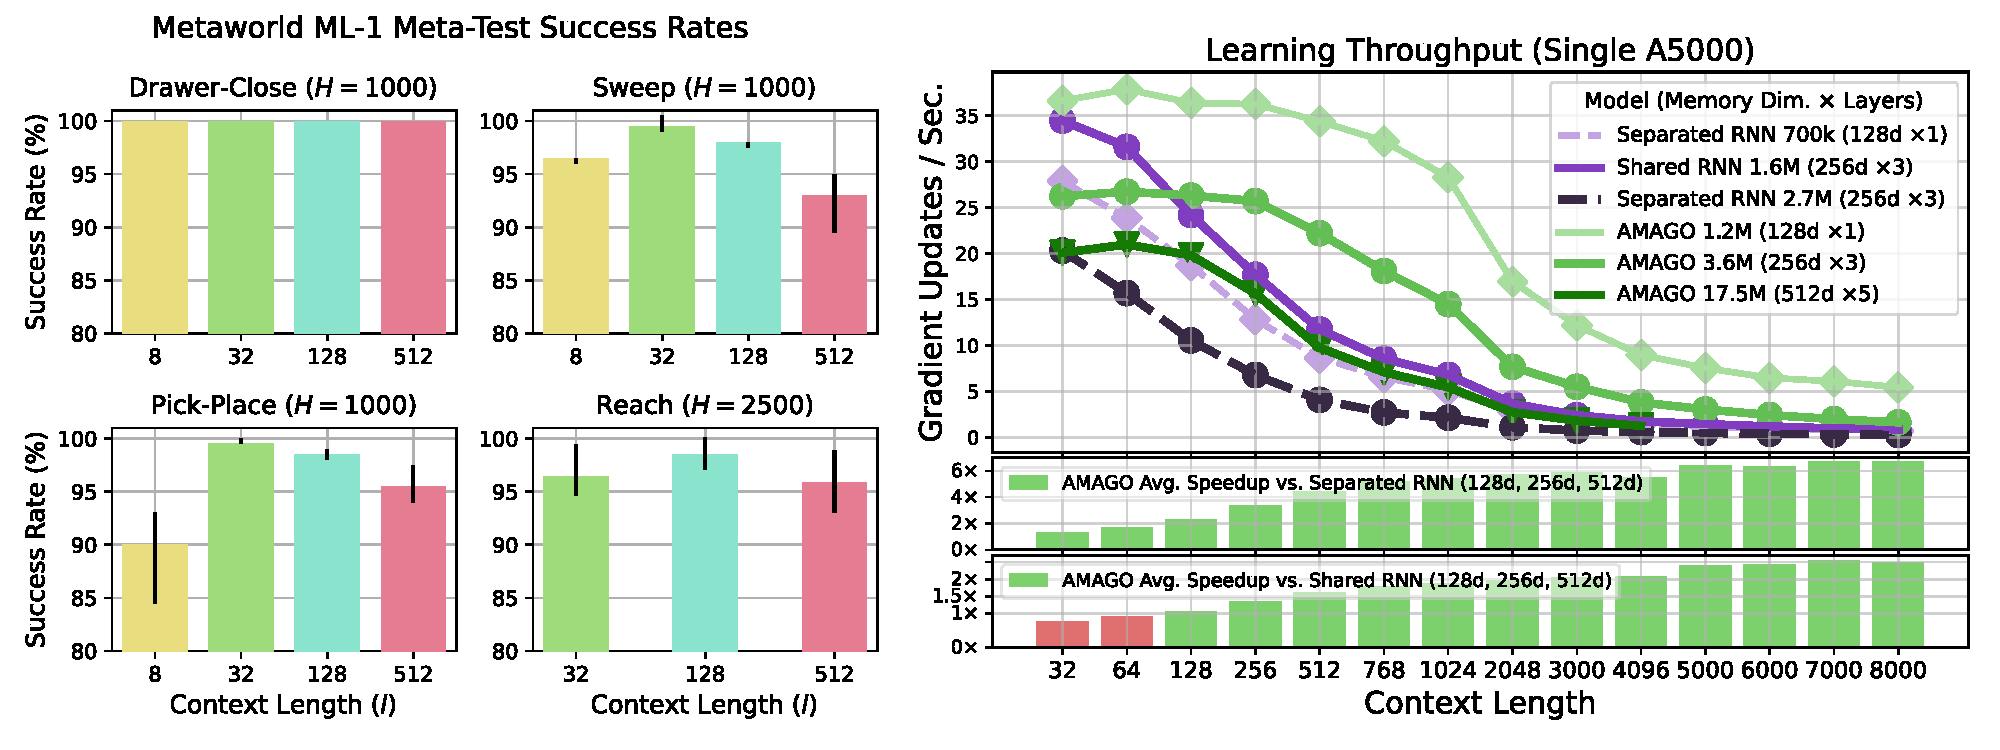
\includegraphics[width=.95\textwidth]{figs/combined_metaworld_throughput.pdf}
    \caption{\textbf{(Left)} Meta-World \cite{yu2020meta} ML-1 success rate on held-out test tasks by context length. \textbf{(Right)} AMAGO enables larger models and longer context lengths than off-policy RNN variants. We compare training throughput in a common locomotion benchmark \cite{finn2017model} with more details in Appendix \ref{app:hparams}.}
    \label{fig:combined_throughput_metaworld}
    \vspace{-3mm}
\end{figure}


Figure \ref{fig:combined_throughput_metaworld} (left) breaks from our default context length $l=H$ and evaluates varying lengths on a sample of Meta-World ML-1 robotics environments \cite{yu2020meta}. Meta-World creates meta-RL tasks out of goal-conditioned environments by masking the goal information, which can be inferred from short context lengths of dense reward signals. While the maximum meta-train performance of every context length is nearly identical, the meta-test success rates decrease slightly over long sequences. Extended contexts may encourage overfitting on these smaller environment distributions. Figure \ref{fig:combined_throughput_metaworld} (right) measures the scalability of AMAGO relative to off-policy agents with a separated RNN architecture as well as the more efficient (but previously unstable) shared model. AMAGO lets us train larger models faster than RNNs with equivalent memory capacity. More importantly, Transformers make optimizing these super-long sequences more realistic.


\subsection{Goal-Conditioned Environment Adaptation}


We now turn our focus towards generalization over procedurally generated environments $e \sim p(e)$ and multi-step instructions $(g^0, \dots, g^k) \sim p(g \mid e)$ of up to $k$ goals (Sec. \ref{sec:background}). A successful policy is able to adapt to a new environment in order to achieve sparse rewards of $+1$ for completing each step of its instruction, creating a general instruction-following agent. Learning to explore from sparse rewards is difficult, but AMAGO's long-horizon off-policy learning update lets us relabel trajectories with alternative instructions (Figure \ref{fig:relabel}). Before we scale up to a more complex domain, we introduce two easily-simulated benchmarks. ``Package Delivery'' is a toy problem where agents navigate a sequence of forks in a road to deliver items to a list of addresses. This task is both sparse and memory-intensive, as achieving any reward requires recall of previous attempts. Appendix \ref{app:experiment_details:package} provides a full environment description, and Figure \ref{fig:package_delivery} compares key ablations of AMAGO. Relabeling, memory, and multi-gamma learning are essential to performance and highlight the importance of AMAGO's technical details.

\begin{figure}[h!]
    \centering
    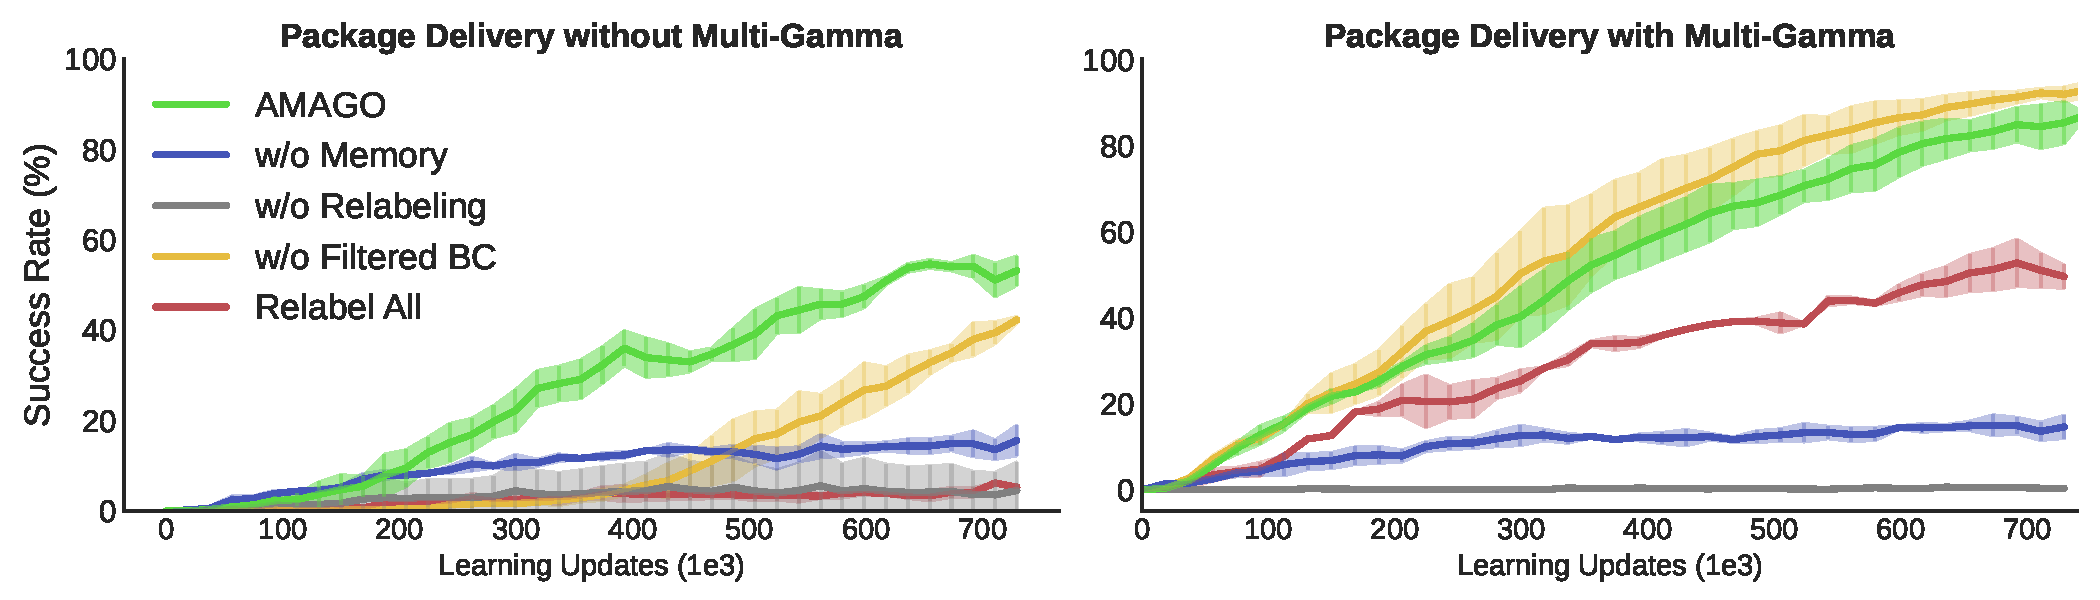
\includegraphics[width=.95\textwidth]{figs/delivery_results_amago_v3.pdf}
    \caption{\textbf{Package Delivery Results.} Relabeling, long-term memory, and multi-gamma updates are essential to success in this sparse goal-conditioned adaptation problem $(H = 180)$.}
    \label{fig:package_delivery}
\end{figure}

\begin{figure}[h!]
    \centering
    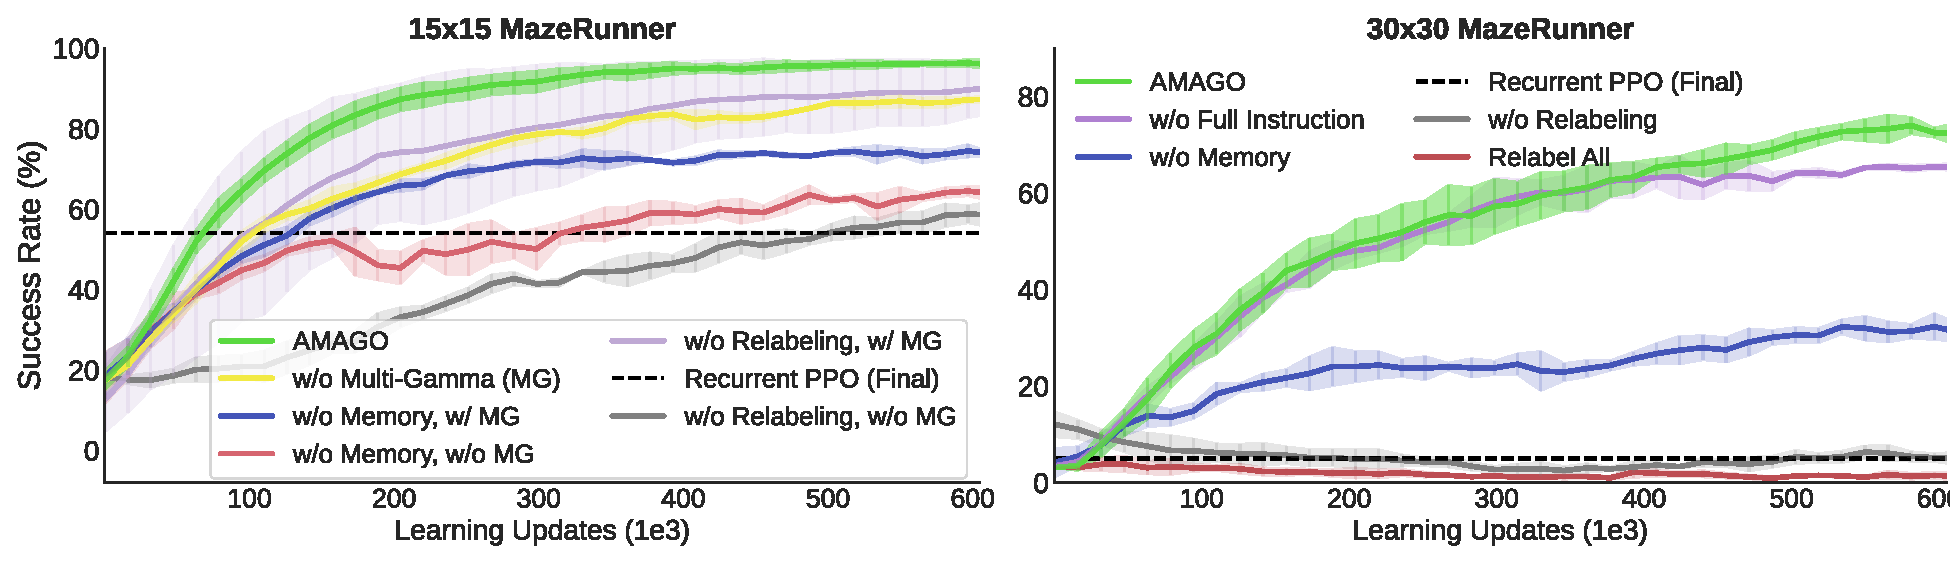
\includegraphics[width=.95\textwidth]{figs/iclr_mazerunner_v1.pdf}
    \caption{\textbf{MazeRunner Results.} Memory improves navigation in a partially observed maze, but sparse rewards create the most significant barrier to learning ($15 \times 15$ $H = 400$, $30 \times 30$ $H = 1,000$).}
    \label{fig:maze_results}
\end{figure}

``MazeRunner'' is a zero-shot maze navigation problem modeled after the example in Figure \ref{fig:relabel} and loosely based on Memory Maze \cite{pasukonis2022evaluating}. The agent finds itself in a familiar spawn location in an otherwise unfamiliar maze and needs to navigate to a sequence of $k \in [1, 3]$ locations. Although the underlying maze map is generated as an $N \times N$ gridworld, the agent's observations are continuous Lidar-like depth sensors. When $N = 15$, the problem is sparse but solvable without relabeling thanks to our implementation's low-level improvements (Figure \ref{fig:maze_results} left). However, $N=30$ is impossibly sparse, and relabeling is crucial to success (Fig. \ref{fig:maze_results} right). We run a similar experiment where action dynamics are randomly reset every episode in Appendix \ref{app:experiment_details:mazerunner}. While this variant is more challenging, our method outperforms other zero-shot meta-RL agents and nearly recovers the original performance while adapting to the new action space.



Crafter \cite{hafner2021benchmarking} is a research-friendly simplification of Minecraft designed to evaluate multi-task capabilities in procedurally generated worlds. Agents explore their surroundings to gather food and resources while progressing through a tech tree of advanced tools and avoiding dangerous enemies. We create an \textit{instruction-conditioned} version where the agent is only successful if it completes the specified task. Our instructions are formed from the $22$ original Crafter achievements with added goals for traveling to a grid of world coordinates and placing blocks in specific locations. Goals are represented as strings like ``make stone pickaxe'', which are tokenized at the word level with the motivation of enabling knowledge transfer between similar goals. Any sequence of $k \leq 5$ goal strings forms a valid instruction that we expect our agent to solve in any randomly generated Crafter environment.

\begin{figure}[h!]
    \vspace{-4mm}
    \centering
    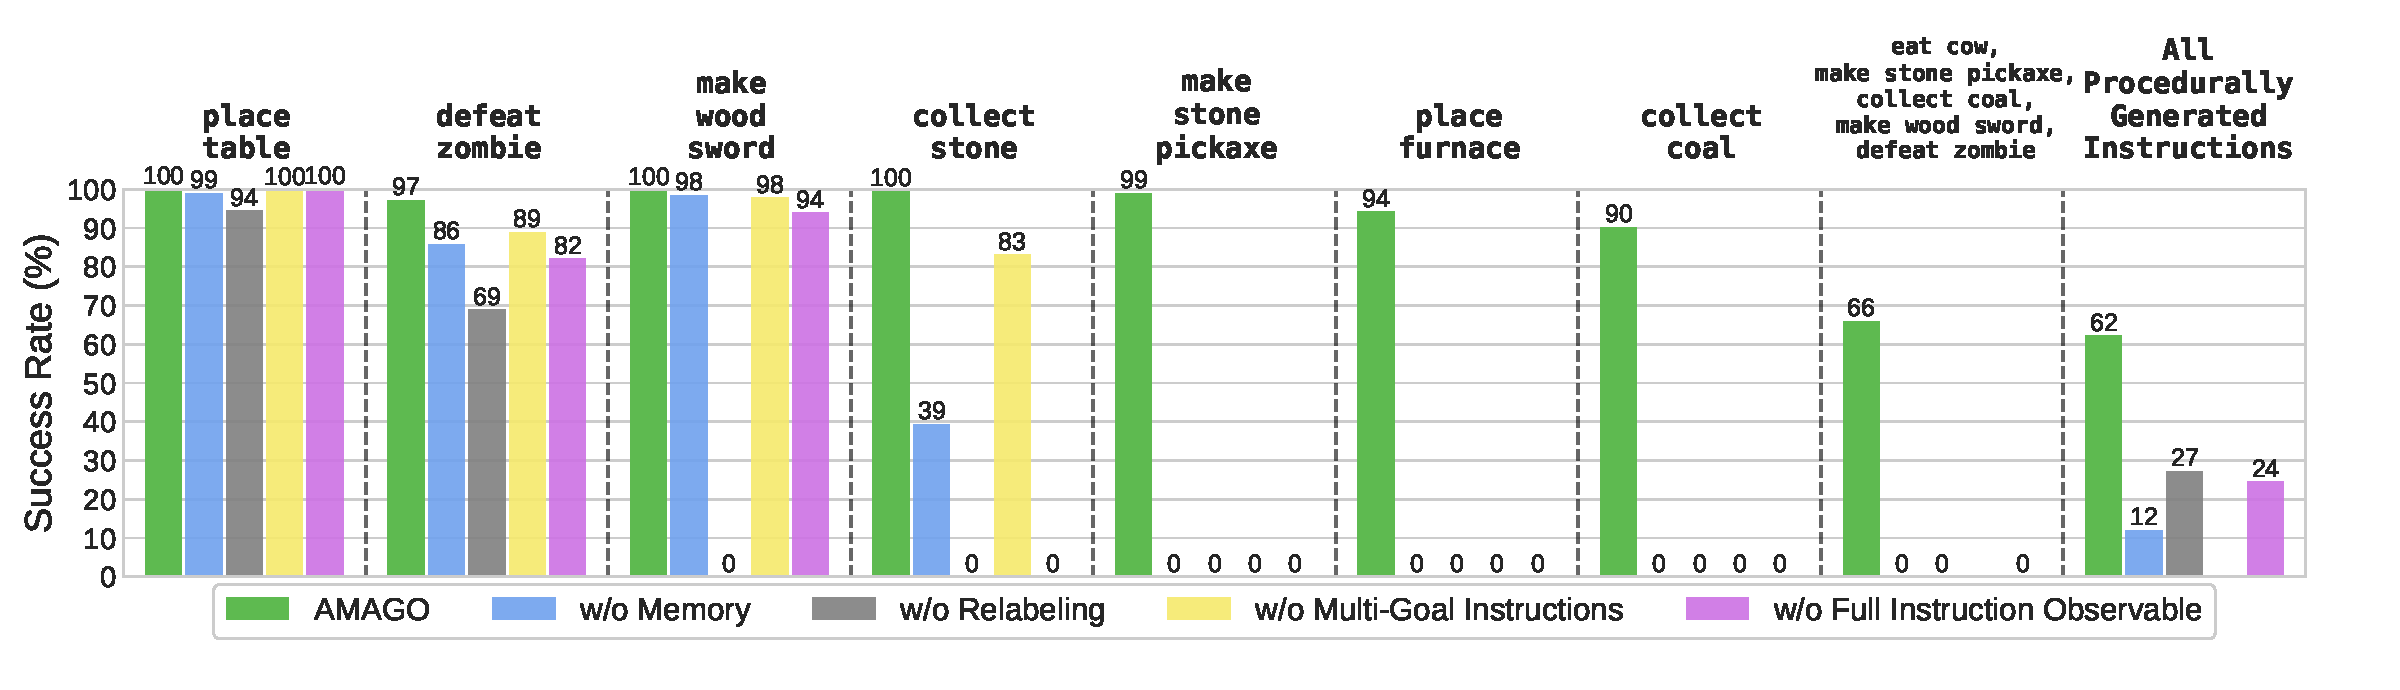
\includegraphics[width=.99\textwidth]{figs/crafter_condensed_results.pdf}
    \vspace{-5mm}
    \caption{\textbf{Crafter Instruction Success Rates.} Here we highlight specific instructions that reveal exploration capabilities. ``All Procedurally Generated Instructions'' indicates performance across the entire range of multi-step goals in randomly generated worlds. \vspace{-2mm}}
    \label{fig:crafter_condensed_results}
\end{figure}

Figure \ref{fig:crafter_condensed_results} shows the success of AMAGO on the entire goal distribution along with several highlighted tasks. Resource-acquisition and tool-making tasks that require test-time exploration and adaptation to a new world benefit from Transformer policies and long-term memory. As the steps in an instruction become less likely to be achieved by random exploration, relabeling becomes essential to success. However, Crafter reveals a more interesting capability of our multi-step hindsight relabeling. If we ablate our relabeling scheme to single-goal HER and evaluate on instructions with length $k=1$ (Fig. \ref{fig:crafter_condensed_results} ``w/o Multi-Goal...''), we find AMAGO loses the ability to complete advanced goals. Crafter's achievement system locks skills behind a progression of prerequisite steps. For example, we can only make tools after we have collected the necessary materials. Relabeling with instructions lets us follow randomly generated sequences of goals we have mastered until we reach the ``frontier'' of skills we have discovered, where new goals have a realistic chance of occurring by random exploration. The agent eventually learns to complete new discoveries as part of other instructions, creating more opportunities for exploration. However, this effect only occurs when we provide the entire task in advance instead of revealing the instruction one step at a time (Fig. \ref{fig:crafter_condensed_results} ``w/o Full Instruction...''). We continue this investigation in detail with additional Crafter experiments in Appendix \ref{app:experiment_details:crafter}.
